\chapter{Plan du Système}
\section{Interactions}
\paragraph{} Le projet est composé d'un web service, d'un client PHP, d'un client Java, d'une base de données et d'une application de gestion.\\
Les clients Java et PHP envoient des requêtes SOAP afin de demander des informations sur des pays.\\
Le web service reçoit les requêtes et les traite en envoyant une requête sur la base de données à l'aide de JDBC.\\
La base de données envoie une réponse et le web service utilise SOAP pour envoyer cette réponse aux clients.\\
L'application de gestion permet à un administrateur de se connecter directement à la base de données pour ajouter, supprimer ou modifier un pays manuellement dans la base de données.\\

\vspace{1.0cm}
\begin{figure}[H]
  \centering
    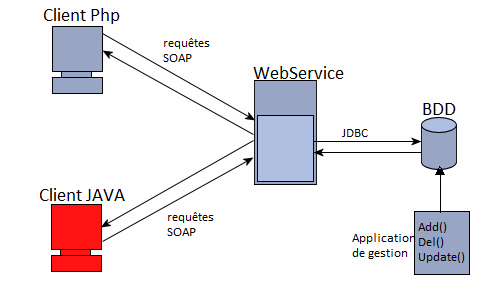
\includegraphics[height= 10cm, width=15cm]{project/images/webservice2}
  \caption{\textbf{Schéma WebService}}
\end{figure}